%---------------------------------------------------------------------------------------
% Propuesta de solución
%
%---------------------------------------------------------------------------------------
\DocumentMetadata{lang=es-MX}
\documentclass[stu,12pt,floatsintext,draftfirst,spanish]{report}

%-----------------------------------------PAQUETES--------------------------------------
\usepackage[spanish,mexico]{babel}
\usepackage[utf8]{inputenc}
\usepackage{times}
\usepackage{physics,amsmath,amssymb,siunitx,codehigh,cancel,float}
\usepackage{hyperref}
\usepackage{csquotes,ragged2e}
\usepackage{tabularray}
\UseTblrLibrary{booktabs}
\usepackage[x11names]{xcolor}
\usepackage{graphicx}
\usepackage[style=apa,sortcites=true,sorting=nyt,backend=biber]{biblatex}
%\addbibresource{referencias.bib}

\DeclareLanguageMapping{spanish}{spanish-apa}

%-------------------------------ESPECIFICACIONES DEL PDF--------------------------------
\hypersetup{
colorlinks=false,
pdfhighlight=/O,
pdfauthor={Jocelyn Janet Parés Ramos},
pdftitle={Propuesta de},
pdfsubject={ASUNTO DEL PDF},
pdfkeywords={PALABRAS CLAVE},
pdfproducer={LaTeX con hyperref},
pdfcreator={pdfLaTeX},
pdfstartview={Fit},
pdfpagemode={UseOutlines},
pdfnewwindow=true,
pdfpagetransition= R,
pdflang=es-MX,
}

%PORTADA--------------------------------------------------------------------------------
\title{Propuesta de solución}
\author{Jocelyn Janet Parés Ramos & 
        Juan Pablo de la Vega Lozano &
        Carlos Alberto Torre Sánchez &
        Ana Camila Murillo Fernández &
        Gael García Zúñiga}
\date{11 de abril, 2025}



%-----------------------------------------DOCUMENTO-----------------------------------------
\begin{document}
\maketitle 

El problema que pensamos resolver es el [\dots.]
 
Nuestra estrategia para resolver el problema es el modelar el sistema de John Deere con el modelo HX10 con 2 cuchillas. Primero, se debe de hacer un análisis de la situación actual del sistema, para después hacer un análisis de los parámetros que se tienen que considerar para el modelo. Las cuchillas funcionan de la siguiente manera:

\begin{figure}[H]
   \centering
   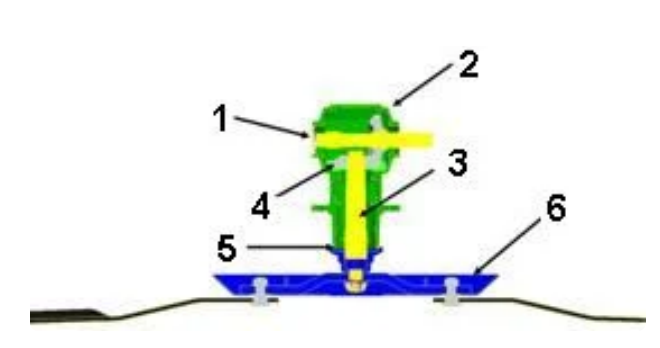
\includegraphics[width=0.5\textwidth]{Blades.png} 
\end{figure}
Las variables que tendríamos que considerar son:
\begin{itemize}
    \item La fuerza producida por el motor
    \item La fuerza 
    \item La eficiencia del motor
    \item 
\end{itemize}
Por lo que haciendo un diagrama de fuerzas obtendriamos lo siguiente:


Estrategia para resolver el problema

Prepara un documento de máximo dos páginas, describiendo la estrategia que usarán para resolver el problema.

Incluye los siguientes puntos:

Define el modelo que utilizarás. Usa figuras y diagramas para explicar tu estrategia.
Define el investiga parámetros realistas para el modelo. No tienen que ser exactos, pero tienen que estar anclados en la realidad.
Define cantidades a modelar y las ecuaciones que las gobiernan.
Explica que estrategias usarán para resolver el problema.
 Modelo 

 Parámetros

 Cantidades y Ecuaciones

 Estrategias
%REFERENCIAS----------------------------------------------------------------------------

%\printbibliography

\end{document}

